\documentclass{modeleRapport}

\addbibresource{biblio.bib}
\usepackage{lmodern}
\hbadness=100000
\vbadness=100000
\scrollmode % Send warning to logs not to show them upon compiling

%--------------------------------------

\titre{Green AI}
\soustitre{A Study About Paris' Air Pollutants}

\enseignant{Nathan \textsc{ELBAZ} \\
            Ali  \textsc{MOKH} \\
}

\eleves{Nour \textsc{AFFES} \\
        Lucas BLANCHET \\
        Hugo BONNELL \\
        Ryan HAMADEH \\
        Yasmine MAARBANI \\
}

%--------------------------------------

\begin{document}

\fairepagedegarde
\fairetabledesmatieres

%--------------------------------------
\section{Introduction}

Air pollution is a pressing environmental issue that affects the health and well-being of millions of people worldwide. In 
urban areas, such as Paris, the impact of pollutants like particulate matter (PM10), nitrogen oxides (NO, NO2, NOX), 
and ozone (O3) is especially critical due to the high population density and traffic congestion. Understanding the trends, 
sources, and behavior of these pollutants is essential for formulating effective policies and strategies to improve air quality 
and mitigate the risks posed by air pollution.\\

This study, conducted as part of the "Green AI" course, focuses on the temporal and chemical dynamics of air pollutants 
in Paris, specifically using data from the air quality monitoring station located in the 18th arrondissement. The dataset, 
which spans from 2018 to the present, provides valuable insights into the concentrations of key pollutants in the city. 
By examining this data, we aim to identify trends, patterns, and correlations that can inform better public health 
and environmental policies.\\

The study is structured around several key areas of analysis. First, we explore the temporal trends of pollutants to 
determine whether their concentrations have been increasing or decreasing over the years, and investigate seasonal 
patterns and daily cycles that influence air quality. We also examine the potential impact of specific policies and events 
on pollutant levels, such as the implementation of low-emission zones or the reduction in activity during the COVID-19 
lockdowns.\\

Another important aspect of the study is the exploration of inter-pollutant relationships, where we analyze the chemical 
and atmospheric interactions between pollutants like NO2 and O3, or NO and NOX. These interactions can provide deeper 
insights into the causes of pollution and help identify critical thresholds at which one pollutant’s increase significantly 
influences the concentration of others.\\

To further enrich our analysis, we conduct comparative studies by benchmarking Paris’s air quality against other major 
cities around the world, providing a contextual understanding of how the city fares in terms of pollution levels. 
Additionally, we explore event-based analyses to assess the impact of specific occurrences, such as public holidays, 
protests, or transportation strikes, on pollutant levels.\\

Finally, in line with modern advancements in data science, we apply machine learning techniques to develop predictive 
models that can forecast pollutant levels based on historical data. This approach will provide a better understanding 
of future pollution patterns and help inform decision-making.\\

By combining data-driven insights with a comprehensive understanding of pollution dynamics, this study aims to contribute 
to the broader conversation about air quality in urban environments and its effects on public health and the environment.



\subsection{Presenting the pollutants}


\subsubsection{PM10 : Particular Matter}

\textbf{Overview:}\\

\begin{itemize}
    \item \textbf{Sources:} Combustion (vehicles, industries), construction dust, agricultural activities, 
    and natural sources like pollen or sea spray.
    \item \textbf{Behaviour:} Particles remain airborne and can travel long distances. They act as surfaces 
    for chemical reactions involving gaseous pollutants.
    \item \textbf{Health impact:} Penetrates the respiratory system, causing cardiovascular and respiratory diseases.\\
\end{itemize}

\textbf{What is it ?}\\

PM10 refers to particulate matter with a diameter of 10 micrometers or less. These fine particles are primarily produced 
from combustion processes (e.g., vehicles and industrial activities), construction dust, agricultural activities, 
and natural sources such as pollen and sea spray. Due to their small size, PM10 particles can remain suspended in the air 
for extended periods, potentially traveling over long distances. They act as surfaces for chemical reactions involving 
gaseous pollutants, including nitrogen oxides and volatile organic compounds. PM10 is a significant concern for human health, 
as it can penetrate deep into the respiratory system, leading to cardiovascular and respiratory diseases, particularly in 
vulnerable populations such as children and the elderly.\\


\subsubsection{NO : Nitric Oxide}

\textbf{Overview:}\\

\begin{itemize}
    \item \textbf{Sources:} Emitted directly from combustion processes in vehicles and power plants.
    \item \textbf{Behaviour:} A reactive gas that plays a key role in forming NO2 and other nitrogen oxides.
    \item \textbf{Health impact:} Precursor to NO2 and ozone (O3) formation.\\
\end{itemize}

\textbf{What is it ?}\\

Nitric oxide (NO) is a colorless and odorless gas primarily emitted from combustion processes, 
including vehicle engines, power plants, and industrial facilities. It plays a crucial role in atmospheric chemistry, 
particularly in the formation of nitrogen dioxide (NO2) and ozone (O3). NO is highly reactive and can quickly react with 
other compounds, making it a key precursor in the production of secondary pollutants. In urban areas, NO levels are closely 
associated with traffic emissions, and its concentration tends to be higher in the colder months when heating and combustion 
activities peak. Though it is not directly harmful in low concentrations, its role in the formation of smog and acid rain 
underscores its importance in air quality studies.\\


\subsubsection{NO2 : Nitrogen Dioxide}

\textbf{Overview:}\\

\begin{itemize}
    \item \textbf{Sources:} Oxidation of NO in the atmosphere; direct emissions from diesel engines and industrial activities.
    \item \textbf{Behaviour:} A toxic gas contributing to smog formation and secondary particulate matter.
    \item \textbf{Health impact:} Contributes to acid rain and ozone production.\\
\end{itemize}

\textbf{What is it ?}\\

Nitrogen dioxide (NO2) is a reddish-brown gas that forms primarily through the oxidation of nitric oxide (NO) in the 
atmosphere. Major sources of NO2 include diesel engines, industrial processes, and power plants. This toxic gas is a key 
component of urban air pollution, contributing to the formation of ground-level ozone and photochemical smog. NO2 is also 
a precursor to acid rain, which can have harmful effects on ecosystems and infrastructure. Additionally, NO2 contributes to 
the formation of secondary particulate matter, worsening air quality. Long-term exposure to elevated NO2 levels is linked to 
respiratory diseases, particularly in children and individuals with pre-existing lung conditions.\\


\subsubsection{NOX : Nitrogen Oxides}

\textbf{Overview:}\\

\begin{itemize}
    \item \textbf{Sources:} Collective term for NO and NO2. Mainly produced from combustion.
    \item \textbf{Behaviour:} Highly reactive, leading to the formation of ozone and nitrates.
    \item \textbf{Health impact:} Major contributor to photochemical smog and secondary aerosol formation.\\
\end{itemize}

\textbf{What is it ?}\\

NOX refers to the collective group of nitrogen oxides, primarily NO and NO2, which are produced during combustion processes 
such as those from vehicles, power plants, and industrial activities. These gases are highly reactive and play a central role 
in atmospheric chemistry, particularly in the formation of ozone and secondary particulate matter. NOX is a major contributor 
to photochemical smog, a key component of urban air pollution, and its presence in the atmosphere leads to the formation of 
nitric acid and nitrates. NOX emissions are also associated with several environmental issues, including acid rain, which 
harms aquatic ecosystems and soil quality. Due to its significant role in air pollution, controlling NOX emissions is 
essential for improving urban air quality and mitigating its harmful effects on human health.\\


\subsubsection{O3 : Ozone}

\textbf{Overview:}\\

\begin{itemize}
    \item \textbf{Sources:} Not emitted directly. Formed by photochemical reactions involving NOX and volatile organic compounds 
    (VOCs) in the presence of sunlight.
    \item \textbf{Behaviour:} A secondary pollutant that peaks during sunny days.
    \item \textbf{Health impact:} Toxic to plants, humans, and animals. A greenhouse gas in the troposphere.\\
\end{itemize}

\textbf{What is it ?}\\

Ozone (O3) is a secondary pollutant that forms in the atmosphere through photochemical reactions involving nitrogen 
oxides (NOX) and volatile organic compounds (VOCs) under the influence of sunlight. Unlike stratospheric ozone, which 
forms the ozone layer and protects life from harmful ultraviolet radiation, ground-level ozone is harmful to human health 
and the environment. Ozone exposure can cause respiratory problems, aggravate asthma, and lead to premature death in 
individuals with cardiovascular conditions. It is also toxic to plants, reducing crop yields and forest productivity. 
Ozone levels typically peak during sunny days and are closely linked to the concentration of precursor pollutants like 
NOX and VOCs, making it a significant focus for air quality monitoring and regulatory efforts.\\


\newpage
\subsection{Review of Related Research}

Before conducting our analysis, we reviewed several key studies that provided valuable context and methodologies 
for understanding urban air pollution. These studies have informed our approach and highlight various challenges, 
opportunities, and solutions in air quality monitoring and forecasting:\\

\begin{enumerate}
    \item \textbf{Methods for Urban Air Pollution Measurement and Forecasting: Challenges, Opportunities, and Solutions.} \cite{UrbanAirPollutionMeasurement}\\
    This study explores the methodologies used for air pollution measurement and forecasting in urban environments. 
    It provides an in-depth analysis of the challenges involved, such as sensor calibration, data sparsity, and the 
    integration of real-time measurements, while proposing advanced solutions like machine learning models 
    and IoT-based monitoring. It guided our understanding of both traditional and modern approaches to air quality monitoring, 
    helping us design a robust methodology for analyzing temporal trends and pollutant interactions.\\
    \item \textbf{Paris Air Quality Monitoring for the 2024 Olympics and Paralympics.} \cite{ParisOlympicsPollutants}\\
    This research focuses on air quality monitoring in Paris in preparation for the 2024 Olympic Games. 
    It highlights the importance of targeted interventions to reduce pollution during large-scale events and evaluates 
    monitoring efforts in urban areas with high population densities.This study was particularly useful in understanding 
    the role of localized monitoring stations and the impact of event-specific air quality interventions.\\
    \item \textbf{Long-term Time-Series Pollution Forecast Using Statistical and Deep Learning Methods.} \cite{PollutantsForecase}\\
    This paper examines the use of statistical and machine learning models for long-term air pollution forecasting. 
    It compares the performance of different methods, including ARIMA and deep learning architectures, 
    in predicting pollutant concentrations. The insights from this study informed our machine learning 
    approach to forecasting pollutant levels based on historical data, particularly in identifying trends 
    and seasonal variations.\\
\end{enumerate}

These foundational studies provided critical context and inspired many aspects of our methodology, 
including temporal analyses, seasonal pattern recognition, and the application of machine learning 
models to forecast pollution levels.\\



%--------------------------------------
\newpage
\section{Temporal Analysis}

\subsection{Trend Analysis}

In this section, we explore the long-term trends in pollutant concentrations from 2018 to 2024 to assess whether levels 
of key pollutants (PM10, NO2, NO, NOX, and O3) have been rising or falling over time. Using linear regression plots, 
the trends for each pollutant have been clearly visualized.\\

\begin{center}
    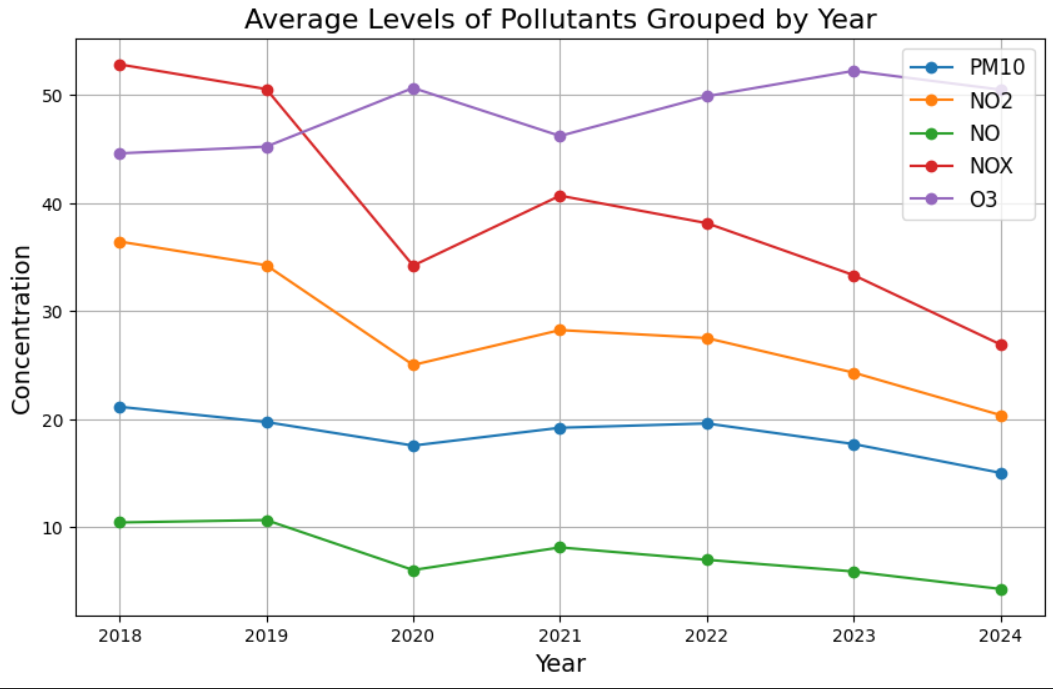
\includegraphics[width=12cm]{Images/PollutantsPerYear.png}
\end{center}

\begin{enumerate}
    \item \textbf{Decreasing Trends: }\\
    PM10, NO2, NO, and NOX: These pollutants exhibit a significant downward trend across the years. 
    This decline may reflect improvements in air quality due to enhanced emission controls, stricter regulations, 
    and technological advancements in vehicle emissions.\\
    \item \textbf{Increasing Trend:}\\
    Ozone (O3): Contrary to the declining trends observed for other pollutants, ozone levels have steadily increased 
    from 2018 to 2024. This rise could be linked to complex photochemical reactions, where reductions in precursors 
    such as NOX might inadvertently enhance O3 formation.\\
    \item \textbf{Impact of Covid19:}\\
    A dramatic drop in NO, NO2, and NOX concentrations occurred in 2020, coinciding with the onset of the COVID-19 pandemic. 
    Reduced traffic and industrial activity during lockdowns contributed to this temporary improvement in air quality.\\
\end{enumerate}


\subsection{Seasonal Patterns}

Analyzing seasonal variations reveals how pollutant concentrations vary by time of year. 
These insights highlight the influence of factors such as weather, human activity, and photochemical 
reactions on pollutant levels.\\

\begin{center}
    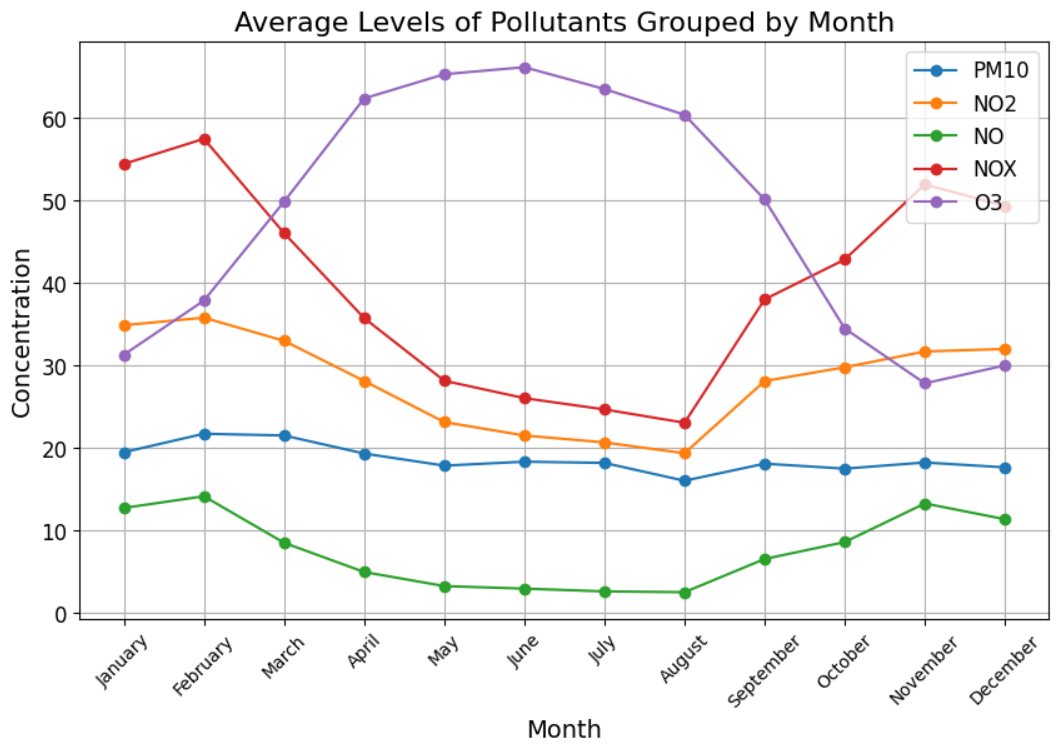
\includegraphics[width=10cm]{Images/PollutantsPerMonth.png}
\end{center}

\begin{enumerate}
    \item \textbf{Ozone (O3):}\\
    It peaks during the spring and summer months, driven by higher sunlight intensity and temperatures that promote ozone 
    formation via photochemical reactions. Levels drop significantly in the winter months, when sunlight is weaker, 
    and temperatures are lower.\\
    \item \textbf{NO, NO2, and NOX:}\\
    They show elevated levels during the colder months, attributed to increased emissions from residential heating systems 
    and reduced atmospheric dispersion due to thermal inversions. Levels decrease in the summer months, when less heating 
    is required, and pollutant dispersion improves.\\
    \item \textbf{PM10:}\\
    PM10 exhibits relatively stable levels throughout the year, with only minor fluctuations. This suggests consistent 
    sources like construction activities, soil dust, and background pollution. Slight increases may occur in winter due to 
    residential heating or reduced atmospheric mixing.\\
    \item \textbf{Impact of Covid19:}\\
    During the 2020 lockdowns, typical seasonal peaks in pollutants like NOX were less pronounced, 
    especially in colder months, as anthropogenic emissions plummeted.\\
\end{enumerate}

\subsection{Time of day}

Daily cycles provide insights into pollution dynamics across a 24-hour period, helping to identify peak pollution hours 
and their associated sources.\\

\begin{center}
    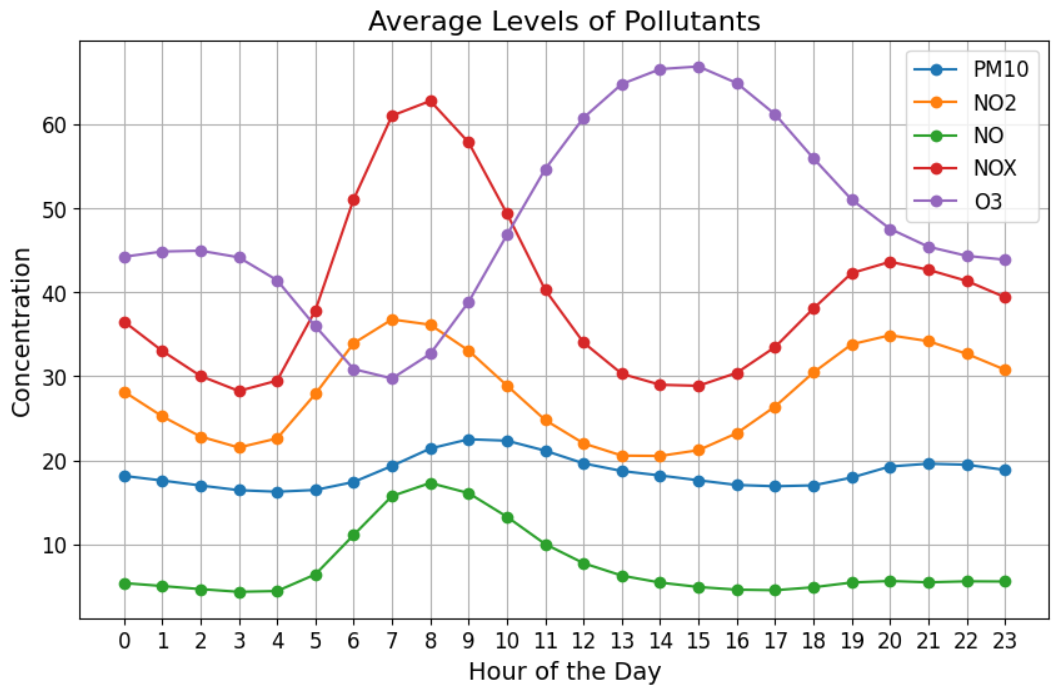
\includegraphics[width=10cm]{Images/PollutantsPerDay.png}
\end{center}

\begin{enumerate}
    \item \textbf{NO, NO2 and NOX:}
    \begin{itemize}
        \item Morning Peak (6–9 AM): Levels surge during morning rush hours due to vehicular emissions and the 
        start of daily human activities.
        \item Evening Peak (5–8 PM): A smaller secondary peak is observed during the evening rush hour, as traffic increases again.
        \item Nighttime Dip: Levels drop sharply at night (11 PM–4 AM), reflecting reduced human activity, emissions, and cooler temperatures 
        that suppress pollutant formation.\\
    \end{itemize}
    \item \textbf{Ozone (O3):}
    \begin{itemize}
        \item Afternoon Peak (1–4 PM): Ozone levels are highest in the afternoon when sunlight is most intense, enabling photochemical 
        reactions that form ozone from precursors like NO2.
        \item Nighttime Minimum: Ozone levels decline at night due to the absence of sunlight and increased titration by NO, 
        a process that converts O3 back to oxygen (O2). (See Chemical reactions section.)\\
    \end{itemize}
    \item \textbf{PM10:}
    \begin{itemize}
        \item Relatively stable throughout the day: PM10 concentrations remain consistent, with no sharp peaks. 
        This stability suggests persistent sources such as construction dust, long-range transport, or background pollution, which are less 
        influenced by diurnal human activities.\\
    \end{itemize}
\end{enumerate}

%--------------------------------------
\section{Policy Impact}


%--------------------------------------
\newpage
\section{Inter-Pollutant Relationships}

\subsection{Chemical Interactions and Relationships}

\subsubsection{Chemical Reactions of PM10}

PM10 particles themselves do not directly participate in chemical reactions in the atmosphere, but they play a crucial 
role in facilitating reactions between gaseous pollutants. Due to their large surface area, PM10 particles can adsorb 
and react with gases like sulfur dioxide (SO2), nitrogen oxides (NOX), and volatile organic compounds (VOCs). 
This results in the formation of secondary pollutants, including sulfate and nitrate particles.
Moreover, PM10 particles can serve as carriers for harmful metals, such as lead and mercury, which have significant 
environmental and health impacts.\\

\subsubsection{Chemical Reactions of NO}

Nitric oxide (NO) is a highly reactive molecule that plays a central role in atmospheric chemistry. NO is primarily 
produced through combustion, where nitrogen in the air reacts with oxygen at high temperatures. Once released into 
the atmosphere, NO can quickly react with ozone (O3) to form nitrogen dioxide (NO2), a process that is often referred to as 
\textbf{NO titration.} This reaction reduces the local concentration of ozone:

$$NO + O_3 \Rightarrow NO_2 + O_2$$

NO can also react with other compounds, such as VOCs, in the presence of sunlight to form secondary pollutants like 
ground-level ozone. In addition, NO plays a key role in the formation of acid rain, as it can react with water vapor 
to produce nitric acid (HNO3), which is then deposited into the environment through precipitation.\\

\subsubsection{Chemical Reactions of NO2}

Nitrogen dioxide (NO2) is a product of the oxidation of NO, and it plays a pivotal role in the formation of ground-level 
ozone, particularly in urban environments. NO2 absorbs sunlight and undergoes photolysis, breaking down into NO and an 
oxygen atom (O). This free oxygen atom can then combine with molecular oxygen (O2) to form ozone (O3):

$$NO_2 + hv_{(sunlight)} \Rightarrow NO+O$$
$$O+O_2 \Rightarrow O_3$$

In addition to ozone formation, NO2 is also involved in the creation of particulate matter. NO2 reacts with hydroxyl 
radicals (OH) and water vapor to form nitric acid (HNO3), which can combine with ammonia (NH3) in the atmosphere to form 
ammonium nitrate, a major component of secondary aerosol pollution.\\

\subsubsection{Chemical Reactions of NOX}

NOX, which refers to the combined presence of nitric oxide (NO) and nitrogen dioxide (NO2), is a major driver of both ozone 
and particulate matter formation. In the presence of sunlight, NOX reacts with volatile organic compounds (VOCs) to produce 
ozone through a series of complex photochemical reactions. This process is especially prominent in urban environments with 
high levels of traffic and industrial emissions. The general mechanism for ozone formation involves the following steps:
\begin{enumerate}
    \item NO2 is photolyzed by sunlight to produce NO and atomic oxygen (O), which then reacts with molecular oxygen (O2) 
    to form ozone (O3).
    \item NO combines with ozone in the atmosphere to form NO2, continuing the cycle and contributing to higher 
    concentrations of both NO2 and ozone. Furthermore, NOX also plays a key role in the formation of particulate matter, 
    particularly secondary organic aerosols (SOAs). These aerosols form through the oxidation of VOCs in the presence of NOX, 
    leading to the creation of fine particles that contribute to smog and reduced air quality.\\
\end{enumerate}


\subsubsection{Chemical Reactions of O3 (Ozone)}

Ozone (O3) is a secondary pollutant, meaning it is not directly emitted but rather forms through complex photochemical 
reactions involving nitrogen oxides (NOX) and volatile organic compounds (VOCs) under the influence of sunlight. Ozone 
plays a dual role in the atmosphere, with beneficial effects in the stratosphere and harmful effects at ground level. In the 
troposphere, ozone is a powerful oxidant, capable of reacting with numerous organic and inorganic compounds. This reactivity 
makes it a major player in air pollution.\\

The formation of ozone begins with the photolysis of nitrogen dioxide (NO2), producing NO and an oxygen atom (O). The 
oxygen atom then reacts with O2 to form ozone:

$$NO_2 + hv_{(sunlight)} \Rightarrow NO+O$$
$$O+O_2 \Rightarrow O_3$$

Ozone can also be depleted in the atmosphere by reactions with nitrogen oxides (NO) in a process known as ozone titration
(mentionned earlier):

$$NO + O_3 \Rightarrow NO_2 + O_2$$

This reaction reduces ozone concentrations, particularly in urban areas with high NO emissions. Additionally, ozone is 
highly reactive with organic compounds, and its presence in the lower atmosphere can contribute to the formation of 
secondary particulate matter, such as fine particulate matter (PM2.5), which can have significant health impacts.

\subsection{Takeaways about air chemistry}

The chemical interactions between PM10, NO, NO2, NOX, and O3 reveal a complex web of processes that influence air 
quality and environmental health. NO and NO2 are central to the formation of both ozone and particulate matter, with their 
interactions driving the production of ground-level ozone, which exacerbates smog and contributes to adverse health outcomes. 
Furthermore, particulate matter like PM10 can act as a carrier for other pollutants and facilitate chemical reactions, while 
ozone itself plays a crucial role in both pollutant formation and degradation. Understanding these chemical reactions is 
essential for developing effective strategies to mitigate air pollution and improve urban air quality.

%--------------------------------------
\newpage
\section{Comparative Studies}



%--------------------------------------
\section{Event-based Analysis}




%--------------------------------------
\newpage
\section{Forecasting}

\subsection{Forecasting Pollutant Concentrations for the next 6 months}

In this section of the study, we aim to forecast the concentrations of key air pollutants (PM10, NO2, NO, NOX, and O3) 
for the next six months using the ARIMA model. The ARIMA (AutoRegressive Integrated Moving Average) model is well-suited 
for time series forecasting due to its ability to capture temporal dependencies and trends in sequential data. For 
this analysis, we applied ARIMA with optimized hyperparameters to the historical hourly pollutant data.\\

The code implemented for this forecasting task first defines a function, which uses the ARIMA model to 
forecast pollutant concentrations. The model parameters were set as (50, 1, 10) (Found by tweaking them), where:\\

\begin{itemize}
    \item 50 is the number of lag observations included in the model (AR term),
    \item 1 represents the differencing order (I term) to make the data stationary, and
    \item 10 is the number of lag observations in the moving average model (MA term).\\
\end{itemize}

Using this function, we forecast the concentrations of five pollutants: PM10, NO2, NO, NOX, and O3 for the next six months, 
as shown in the plot below.

\begin{center}
    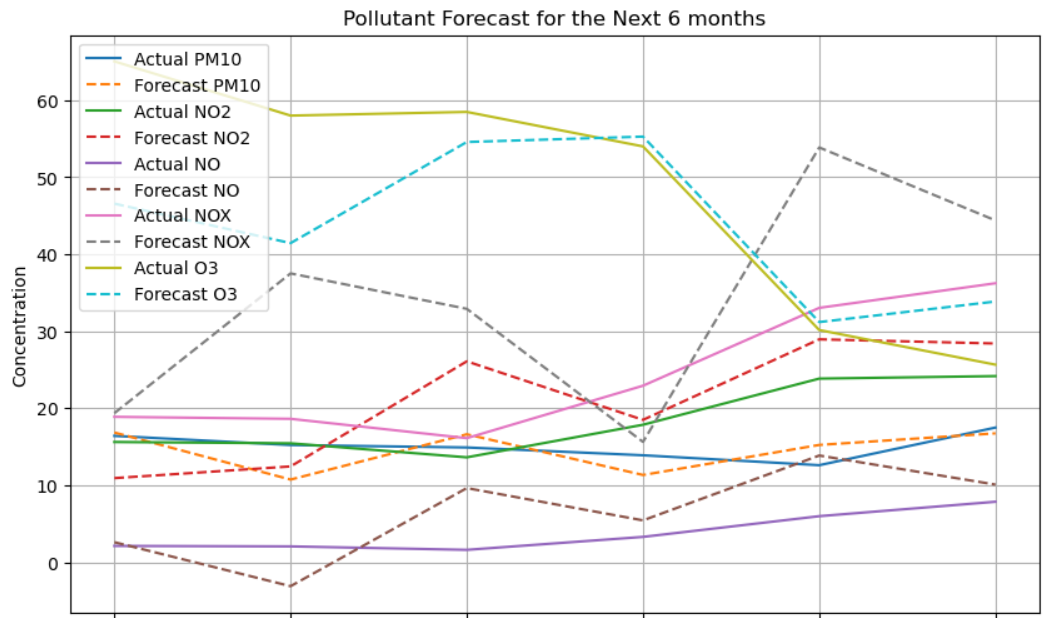
\includegraphics[width=14cm]{Images/PollutantsForecast.png}
\end{center}

\newpage
\subsection{Plotting the Forecast}
The resulting forecasted values (dashed lines) are overlaid with the actual historical values (solid lines) for each pollutant, 
with the date on the x-axis and pollutant concentration on the y-axis. The forecast is conducted on the test dataset, 
which includes actual pollutant concentrations up to the current period.\\

The forecasted trends suggest how each pollutant may evolve in the next 6 months, providing valuable insights into the 
potential future air quality scenario in Paris. For example, pollutants like NOX and O3 exhibit fluctuations that could help 
in formulating effective air quality management strategies.\\

\subsection{Model Evaluation: MAE and RMSE}

To assess the accuracy of the forecast, we calculated the Mean Absolute Error (MAE) and Root Mean Squared Error (RMSE) 
for each pollutant. These metrics provide a quantitative measure of the model's prediction error. The results of the 
evaluation are as follows:\\

\begin{itemize}
    \item MAE PM10: 2.10, RMSE PM10: 2.49
    \item MAE NO2: 5.02, RMSE NO2: 6.20
    \item MAE NO: 4.32, RMSE NO: 5.21
    \item MAE NOX: 12.07, RMSE NOX: 14.10
    \item MAE O3: 8.24, RMSE O3: 10.81
\end{itemize}

These values reflect a reasonable forecast performance, with lower errors for pollutants like PM10 compared to others 
like NOX and O3. The higher errors in NOX and O3 could be due to their greater variability, which is more difficult to 
model accurately with the chosen ARIMA configuration. These errors indicate areas where the model could potentially be 
refined by adjusting parameters or using more advanced forecasting techniques.\\


%--------------------------------------
\newpage
\section{Conclusion}

%--------------------------------------
\insererbiblio

\end{document}